% 编译命令：xelatex main.tex

\documentclass[filled]{zjuthesis}% 填入filled参数，自动填写Checklist表格相关信息
\begin{document}

\zju{
    title = {Medical Reasoning with Memory-Augmented Agentic System},
    name = {Zihan Xu},
    id = {3220110781},
    supervisor = {Zuozhu Liu},
    class of year = {2026},
    major = {Computer Engineering},
    submission date = {May 2026},
    Academic title = {Assistant Professor},
}

\maketitle

\frontmatter

\Checklist
\Commitment

{\doublespacing
    \centerline{\xiaoyi\bfseries Acknowledgements}

I would like to express my sincere gratitude to my supervisor, Professor Zuozhu Liu, for his guidance, patience, and insightful feedback throughout the course of this thesis project. His expertise in medical AI and deep learning provided the intellectual foundation upon which this work was built.

I am grateful to my collaborators on the LongMedBench project, whose work on the factual question-answering and temporal reasoning components provided essential context for the decision-making framework developed in this thesis. The collaborative environment fostered productive discussions that sharpened the research questions and methodology.

I also acknowledge the maintainers of the MIMIC-IV database, whose commitment to open clinical data access makes research of this kind possible. The computational resources provided by [TODO: institution/computing platform] were essential for the experimental evaluation.

Finally, I thank my family for their unwavering support throughout my undergraduate studies, and the faculty of the Computer Engineering program at [TODO: university name] for providing a rigorous and inspiring academic environment.

    \centerline{\xiaoyi\bfseries Abstract}

Clinical decision-making is inherently longitudinal — clinicians must synthesize evidence across repeated hospitalizations, diagnostic tests, and evolving treatment responses spanning months or years. However, current benchmarks for medical large language model (LLM) agents predominantly evaluate single-encounter behavior, focusing on tool-use accuracy and fact retrieval rather than the cross-visit temporal integration that real clinical practice demands. This thesis presents the decision-making component of LongMedBench, a benchmark constructed from real-world Electronic Health Record (EHR) data (MIMIC-IV) that evaluates LLM agents on long-horizon clinical decision-making. We design a three-tier memory architecture operating at three granularities — Note Memory (coarse-grained visit summaries), Event Memory (fine-grained structured event sequences), and Contextual Memory (immediate visit context) — and systematically compare memory provision strategies including naive long-context, retrieval-augmented generation (RAG), and agent memory systems (Mem0). Through experiments on GPT-5-mini, DeepSeek-v3.2, and Qwen-Turbo, we find that decision-making accuracy across all models remains modest (approximately 0.55--0.62 exact match), and critically, that memory augmentation architectures provide no significant improvement over the naive long-context baseline. Decision accuracy depends primarily on the immediate clinical context, with historical information contributing negligible marginal value regardless of memory granularity or retrieval strategy. This central finding reveals a retrieval-reasoning gap: current architectures can locate relevant historical facts but cannot effectively integrate them into proactive clinical planning. We discuss the implications of this gap for medical AI agent design and propose directions for memory architectures that go beyond retrieval to support structured longitudinal reasoning.

\vspace{2em}
\noindent\textbf{Keywords:} Medical AI Agents, Clinical Decision-Making, EHR Benchmark, Long-Horizon Reasoning, Memory-Augmented LLM, Retrieval-Augmented Generation
}

\tableofcontents

\mainmatter

\chapter{Introduction}

\section{The Long-Horizon Challenge in Clinical Decision-Making}

Clinical practice is fundamentally longitudinal. Patients with chronic conditions accumulate medical histories spanning years and dozens of hospitalizations, and at each encounter clinicians must synthesize evidence across prior diagnostic tests, imaging studies, medication adjustments, and evolving treatment responses \cite{pmid41325597}. A patient with end-stage renal disease undergoing 18 hospitalizations over two years presents not as a series of isolated episodes, but as a continuous trajectory where each admission's clinical decisions depend on what was learned in prior ones. This capacity for cross-visit temporal integration is central to clinical reasoning, and it represents a capability that medical AI must acquire to be clinically useful.

As large language models (LLMs) transition from static question-answering to autonomous medical agents, their ability to navigate longitudinal clinical trajectories has become a critical benchmark for clinical readiness \cite{PhysioNet-mimiciv-3.1}. Yet existing evaluation paradigms largely fail to capture this temporal dimension. Most benchmarks assess single-encounter behavior: tool-use accuracy in a simulated visit, diagnosis from a single symptom set, or fact retrieval from a single discharge summary. These evaluations, while valuable, do not measure the cross-visit temporal integration that real clinical practice demands.

This thesis presents the decision-making component of \textbf{LongMedBench}, a benchmark constructed from MIMIC-IV EHR data that evaluates LLM agents on long-horizon clinical decision-making. Our work bridges two previously disconnected lines of research: the design of long-horizon interaction benchmarks from the general AI domain, and the evaluation of clinical reasoning from real-world EHR data. Through a three-tier memory architecture and systematic ablation of memory strategies, we investigate a central question: given long-context windows, RAG, and agent memory systems, how well can contemporary LLMs integrate longitudinal clinical history to inform next-step decisions?

\section{Medical Benchmarks for Clinical AI}

Medical AI evaluation has evolved from static QA to interactive agent settings. First-generation benchmarks (MedBench \cite{2023_medbench}, PromptCBLUE \cite{2023_promptcblue}) tested knowledge recall from medical licensing exams. Second-generation work introduced real clinical data: EHRSQL \cite{lee2022ehrsql} pioneered text-to-SQL on structured EHR; FHIR-AgentBench \cite{2025_fhir_agentbench} extended this to interoperable FHIR standards; MedAlign \cite{2024_medalign} provided clinician-generated instruction-following tasks grounded in EHR data.

Third-generation interactive agent benchmarks now dominate. MedAgentBench \cite{jiang2025medagentbench} introduced a virtual EHR environment with 300 clinician-written tasks. AgentClinic \cite{schmidgall2025agentclinicmultimodalagentbenchmark} added multimodal clinical encounters. ER-REASON \cite{2025_er_reason} focused on emergency room reasoning with structured subtasks. MedAgentGym \cite{2025_medagentgym} provided a scalable training environment for biomedical reasoning. Comprehensive evaluation suites like MedHelm \cite{2026_medhelm}, HealthBench \cite{2025_healthbench}, and BRIDGE \cite{2025_bridge} aggregate diverse tasks for holistic assessment.

Despite this progress, a critical gap persists: all current medical benchmarks evaluate \emph{single-encounter} behavior. Real clinical care spans dozens of visits over years, and a patient's current presentation cannot be understood in isolation from their clinical trajectory. Even agent-based benchmarks (MedAgentBench, AgentClinic) are bounded to one visit. EHR-Bench \cite{2025_ehr_r1} is the closest precedent---derived from MIMIC-IV with 42 tasks spanning multi-visit trajectories---but its formulation is static (predict the next event from a complete history), closer to classification than interactive agent decision-making. Most importantly, no existing medical benchmark systematically compares \emph{memory architectures} (long-context vs.\ retrieval vs.\ agent memory) for clinical decision-making.

Table~\ref{tab:med_bench} provides a systematic comparison along dimensions critical to longitudinal clinical AI.

\begin{table}[!h]
    \centering
    \caption{Comparison of medical benchmarks for clinical AI.}
    \label{tab:med_bench}
    {\fontsize{8}{9.5}\selectfont
    \setlength{\tabcolsep}{2pt}
    \renewcommand{\arraystretch}{1.1}
    \begin{tabular*}{\textwidth}{>{\raggedright\arraybackslash}m{0.18\textwidth}>{\centering\arraybackslash}m{0.07\textwidth}>{\centering\arraybackslash}m{0.08\textwidth}>{\centering\arraybackslash}m{0.07\textwidth}>{\centering\arraybackslash}m{0.08\textwidth}>{\centering\arraybackslash}m{0.08\textwidth}>{\centering\arraybackslash}m{0.09\textwidth}>{\centering\arraybackslash}m{0.08\textwidth}>{\centering\arraybackslash}m{0.14\textwidth}}
        \toprule
        \textbf{Benchmark} & \textbf{EHR} & \textbf{Multi-Visit} & \textbf{Agent} & \textbf{Decision-Making} & \textbf{Temporal} & \textbf{Memory Study} & \textbf{Year} & \textbf{Data Source} \\
        \midrule
        MedBench \cite{2023_medbench} & & & & & & & 2023 & Exams \\
        PromptCBLUE \cite{2023_promptcblue} & & & & & & & 2023 & Exams \\
        EHRSQL \cite{lee2022ehrsql} & \checkmark & & & & & & 2022 & MIMIC-IV \\
        MedAlign \cite{2024_medalign} & \checkmark & & & \checkmark & & & 2024 & STARR \\
        MedAgentBench \cite{jiang2025medagentbench} & \checkmark & & \checkmark & & & & 2025 & STARR \\
        AgentClinic \cite{schmidgall2025agentclinicmultimodalagentbenchmark} & \checkmark & & \checkmark & & & & 2025 & Simulated \\
        ER-REASON \cite{2025_er_reason} & \checkmark & & \checkmark & \checkmark & & & 2025 & MIMIC-IV \\
        FHIR-AgentBench \cite{2025_fhir_agentbench} & \checkmark & & \checkmark & & & & 2025 & MIMIC-IV \\
        MedAgentGym \cite{2025_medagentgym} & \checkmark & & \checkmark & & & & 2025 & Multiple \\
        BRIDGE \cite{2025_bridge} & \checkmark & & & & & & 2025 & Multiple \\
        TIMER \cite{2025_timer} & \checkmark & \checkmark & & & \checkmark & & 2025 & STARR \\
        EHR-Bench \cite{2025_ehr_r1} & \checkmark & \checkmark & & \checkmark & & & 2025 & MIMIC-IV \\
        HealthBench \cite{2025_healthbench} & \checkmark & & & & & & 2025 & Multiple \\
        MedHelm \cite{2026_medhelm} & \checkmark & & & & & & 2026 & Multiple \\
        \midrule
        \textbf{LongMedBench} & \checkmark & \checkmark & \checkmark & \checkmark & \checkmark & \checkmark & 2026 & MIMIC-IV \\
        \bottomrule
    \end{tabular*}
    }
\end{table}

\noindent \textit{Legend:} \checkmark = capability present. EHR = real electronic health record data. Agent = interactive agent-based evaluation. Memory Study = systematic memory architecture ablation.

\section{Long-Horizon Benchmarks in the General Domain}

In parallel with medical AI, the general NLP community has developed a rich set of benchmarks targeting long-context understanding and long-horizon interaction. Unlike medical benchmarks, these do not use clinical data, but their \emph{task design principles}---multi-turn interaction, cross-session memory, progressive information revelation---directly inform the construction of longitudinal clinical benchmarks.

\textbf{Long-Context Retrieval Benchmarks.} RULER \cite{hsieh2024rulerwhatsrealcontext} systematically evaluates the effective context window of LLMs through synthetic tasks (needle-in-a-haystack, variable tracking) at controlled lengths up to 128K tokens. NarrativeQA \cite{kočiský2017narrativeqareadingcomprehensionchallenge} tests reading comprehension over full-length books and movie scripts, requiring models to answer questions that depend on information distributed across long documents. These benchmarks established that LLMs can retrieve facts from long contexts, but they do not test whether models can \emph{reason across} temporally structured information---a gap particularly relevant to clinical trajectories.

\textbf{Multi-Hop and Multi-Turn Benchmarks.} HotpotQA \cite{yang2018hotpotqa} requires reasoning across multiple documents to answer questions, introducing the concept of multi-hop reasoning that parallels the clinical need to connect evidence across visits. LoCoMo \cite{loComo_reference} evaluates long-term conversational memory through multi-session dialogues, where models must recall and reason about information shared in earlier sessions---directly analogous to recalling clinical events from prior hospitalizations.

\textbf{Interactive Agent Benchmarks.} TRIP-Bench \cite{shen2026tripbenchbenchmarklonghorizoninteractive} evaluates agents on long-horizon interactive tasks in real-world scenarios, where agents must plan, execute, and adapt across extended interactions. LongMemEval \cite{wu2024longmemeval} specifically targets long-term interactive memory in chat assistants, evaluating whether models can retain and use information shared across multiple dialogue sessions.

Table~\ref{tab:gen_bench} summarizes these benchmarks. The key design pattern they share---structuring evaluation around progressively longer interaction horizons and measuring how performance degrades with distance---directly inspired LongMedBench's visit injection ablation design.

\begin{table}[!h]
    \centering
    \caption{Long-horizon and long-context benchmarks in the general domain.}
    \label{tab:gen_bench}
    {\fontsize{8}{9.5}\selectfont
    \setlength{\tabcolsep}{3pt}
    \renewcommand{\arraystretch}{1.1}
    \begin{tabular*}{\textwidth}{>{\raggedright\arraybackslash}m{0.18\textwidth}>{\centering\arraybackslash}m{0.08\textwidth}>{\centering\arraybackslash}m{0.09\textwidth}>{\centering\arraybackslash}m{0.10\textwidth}>{\centering\arraybackslash}m{0.10\textwidth}>{\centering\arraybackslash}m{0.13\textwidth}>{\centering\arraybackslash}m{0.14\textwidth}}
        \toprule
        \textbf{Benchmark} & \textbf{Multi-Turn} & \textbf{Long Context} & \textbf{Interactive} & \textbf{Reasoning} & \textbf{Key Design} & \textbf{Year} \\
        \midrule
        NarrativeQA \cite{kočiský2017narrativeqareadingcomprehensionchallenge} & & \checkmark & & & Full-book comprehension & 2017 \\
        HotpotQA \cite{yang2018hotpotqa} & & & & \checkmark & Multi-doc reasoning & 2018 \\
        RULER \cite{hsieh2024rulerwhatsrealcontext} & & \checkmark & & & Synthetic context stress test & 2024 \\
        LoCoMo \cite{loComo_reference} & \checkmark & \checkmark & \checkmark & \checkmark & Multi-session dialogues & 2024 \\
        LongMemEval \cite{wu2024longmemeval} & \checkmark & \checkmark & \checkmark & \checkmark & Long-term chat memory & 2024 \\
        TRIP-Bench \cite{shen2026tripbenchbenchmarklonghorizoninteractive} & \checkmark & \checkmark & \checkmark & \checkmark & Real-world interactive planning & 2026 \\
        AMA-Bench \cite{amabench2026} & \checkmark & \checkmark & \checkmark & \checkmark & Memory for agentic applications & 2026 \\
        \bottomrule
    \end{tabular*}
    }
\end{table}

\noindent \textit{Legend:} \checkmark = capability present. Long Context = requires processing contexts exceeding typical window sizes. Interactive = involves multi-step agent-environment interaction.

\section{Memory-Augmented Architectures for Long-Horizon Interaction}

To address the challenges exposed by long-horizon benchmarks, a parallel line of research has developed memory-augmented architectures that extend LLM capabilities beyond their native context windows. These frameworks are not benchmarks themselves, but the \emph{infrastructure} that enables agents to manage information across extended interactions---exactly the capability required for clinical decision-making over years of patient history.

\textbf{Retrieval-Augmented Generation (RAG).} The foundational RAG paradigm \cite{lewis2020rag} augments LLM inference by retrieving relevant documents from an external knowledge base and prepending them to the context window. RAG separates memory storage (the indexed corpus) from inference, enabling scale beyond the context window at the cost of retrieval quality.

\textbf{Agent Memory Systems.} Mem0 \cite{mem0_reference} provides a persistent, evolvable memory layer with add, search, and update operations. MemGPT \cite{memgpt_reference} introduced an OS-inspired memory hierarchy with working and archival storage. More recent frameworks have pushed further: A-MEM \cite{amem2025} explicitly models agentic memory decisions, where the agent autonomously determines what to retain; EverMemOS \cite{evermemos2026} proposes a self-organizing memory operating system for structured long-horizon reasoning; and Memory as Action \cite{memoryasaction2025} reframes memory management as an action the agent takes, integrating it into the decision loop rather than treating it as preprocessing.

\textbf{Context Optimization.} Agentic Context Engineering \cite{zhang2026agentic} learns to compress and organize context. Context-Folding \cite{contextfolding2026} scales long-horizon agents by folding past context into compressed representations, directly addressing the tension between history retention and context window limits.

Table~\ref{tab:memory} summarizes these frameworks chronologically. Despite their architectural diversity, a common assumption underlies them: that \emph{better memory retrieval leads to better task performance}. Whether this assumption holds for proactive clinical decision-making---where retrieval is necessary but not sufficient---is a central question that LongMedBench is designed to answer.

\begin{table}[!h]
    \centering
    \caption{Memory-augmented architectures for LLM agents.}
    \label{tab:memory}
    {\fontsize{8}{9.5}\selectfont
    \setlength{\tabcolsep}{3pt}
    \renewcommand{\arraystretch}{1.1}
    \begin{tabular*}{\textwidth}{>{\raggedright\arraybackslash}m{0.17\textwidth}>{\centering\arraybackslash}m{0.15\textwidth}>{\centering\arraybackslash}m{0.20\textwidth}>{\centering\arraybackslash}m{0.10\textwidth}>{\centering\arraybackslash}m{0.07\textwidth}>{\centering\arraybackslash}m{0.17\textwidth}}
        \toprule
        \textbf{Framework} & \textbf{Strategy} & \textbf{Key Mechanism} & \textbf{Persist.} & \textbf{Year} & \textbf{Innovation} \\
        \midrule
        RAG \cite{lewis2020rag} & Retrieve-then-generate & Embed + Retrieve + Augment & Ext. & 2020 & Separates storage \& inference \\
        MemGPT \cite{memgpt_reference} & Hierarchical memory & Core + Archival paging & \checkmark & 2023 & OS-inspired management \\
        Mem0 \cite{mem0_reference} & Agent memory layer & Add + Search + Update & \checkmark & 2024 & Multi-session persistence \\
        A-MEM \cite{amem2025} & Agentic memory & Autonomous retention & \checkmark & 2025 & Agent-driven memory \\
        Memory as Action \cite{memoryasaction2025} & Memory-as-decision & Context curation loop & \checkmark & 2025 & Memory in decision loop \\
        EverMemOS \cite{evermemos2026} & Self-organizing OS & Structured long-horizon & \checkmark & 2026 & Self-organizing memory \\
        Context-Folding \cite{contextfolding2026} & Context compression & Fold + Compress history & \checkmark & 2026 & Learned history compression \\
        \bottomrule
    \end{tabular*}
    }
\end{table}

\noindent \textit{Legend:} \checkmark = yes. Persistent = memory state survives across sessions/interactions.

\section{LongMedBench: Bridging Two Lines of Research}

LongMedBench is positioned at the intersection of these two bodies of work. On one hand, it inherits the \emph{domain grounding} of medical benchmarks: real EHR data (MIMIC-IV), clinically meaningful action spaces, and ground-truth labels extracted from actual patient records. On the other hand, it adopts the \emph{task design methodology} of general long-horizon benchmarks: progressive context expansion (visit injection ablation), multi-session memory management, and systematic comparison of retrieval architectures.

This dual inheritance makes LongMedBench innovative in both dimensions:

\begin{enumerate}
    \item \textbf{Innovation in medical AI:} LongMedBench is the first benchmark to combine real EHR data with interactive agent evaluation and systematic memory architecture ablation. No prior medical benchmark (Table~\ref{tab:med_bench}) has systematically compared how different memory strategies---naive long-context, retrieval-augmented, and agent-managed memory---affect clinical decision-making.
    
    \item \textbf{Innovation in long-horizon AI:} LongMedBench is the first benchmark to apply long-horizon interaction task design (as developed in NarrativeQA, RULER, LoCoMo, TRIP-Bench) to real-world clinical data. Unlike general-domain benchmarks that use synthetic or curated text, LongMedBench tests long-horizon reasoning on noisy, real-world clinical trajectories with genuine temporal structure and clinical consequence.
\end{enumerate}

The empirical heart of this thesis is a systematic ablation study that evaluates three memory strategies (Naive Long-Context, RAG, Mem0) across three memory granularities (Note, Event, Context) at varying historical depths, using three state-of-the-art LLMs. This design directly addresses the question that neither medical benchmarks nor general long-horizon benchmarks have answered: \emph{do memory-augmented architectures improve clinical decision-making over longitudinal patient trajectories?}

\section{Research Questions}

Specifically, this thesis investigates three questions:

\begin{enumerate}
    \item \textbf{Memory granularity:} Does the format of historical information---structured event-level data vs.\ narrative note-level summaries---affect clinical decision quality?
    \item \textbf{Memory architecture:} Do RAG and agent memory systems (Mem0) improve longitudinal decision-making relative to providing the full history in context?
    \item \textbf{Historical depth:} Does decision performance plateau, improve, or degrade as more historical visits are included?
\end{enumerate}

\section{Contributions}

Within the broader LongMedBench project (whose factual QA and temporal reasoning tasks are undertaken by collaborators), this thesis makes four contributions:

\begin{enumerate}
    \item \textbf{EHR-to-Agent Data Pipeline.} A reproducible pipeline transforming raw MIMIC-IV records into longitudinal event streams for interactive agent evaluation, yielding 355 patients (mean 19.72 visits/patient, 44.91 medical events/visit).
    
    \item \textbf{Three-Tier Memory Architecture.} A memory framework operating at three granularities---Note Memory (coarse-grained visit summaries), Event Memory (fine-grained structured event sequences), and Contextual Memory (immediate visit context)---enabling systematic ablation of memory granularity effects.
    
    \item \textbf{Long-Horizon Decision-Making Task (T3-D).} An interactive evaluation protocol where the agent receives a partial patient trajectory through controlled memory and must predict the next clinical action from a predefined action space, with ground truth extracted from actual clinical records.
    
    \item \textbf{Empirical Finding.} Through experiments across GPT-5-mini, DeepSeek-v3.2, and Qwen-Turbo comparing Naive Long-Context, RAG, and Mem0 strategies, we find that memory augmentation provides \emph{no significant improvement} for longitudinal clinical decision-making. Decision accuracy depends primarily on immediate context, revealing a retrieval-reasoning gap.
\end{enumerate}

\section{Scope and Structure}

This thesis focuses exclusively on T3-D (Decision-Making). The T3-A (Fact-based QA) and T3-N (Temporal Reasoning) tasks are covered in collaborators' separate theses.

Chapter~2 presents the data processing pipeline, three-tier memory architecture, T3-D task design, experimental setup, and results. Chapter~3 discusses the implications of our findings, acknowledges limitations, and outlines future research directions.

\chapter{Methodology and Experiments}

This chapter presents the LongMedBench decision-making pipeline: from raw EHR data to interactive agent evaluation. Section~\ref{sec:pipeline} describes the data processing pipeline. Section~\ref{sec:memory} presents the three-tier memory architecture. Section~\ref{sec:task} formulates the decision-making task. Section~\ref{sec:expsetup} details the experimental design. Section~\ref{sec:results} presents results and analysis.

\section{EHR Data Processing Pipeline}
\label{sec:pipeline}

\begin{figure}[ht]
    \centering
    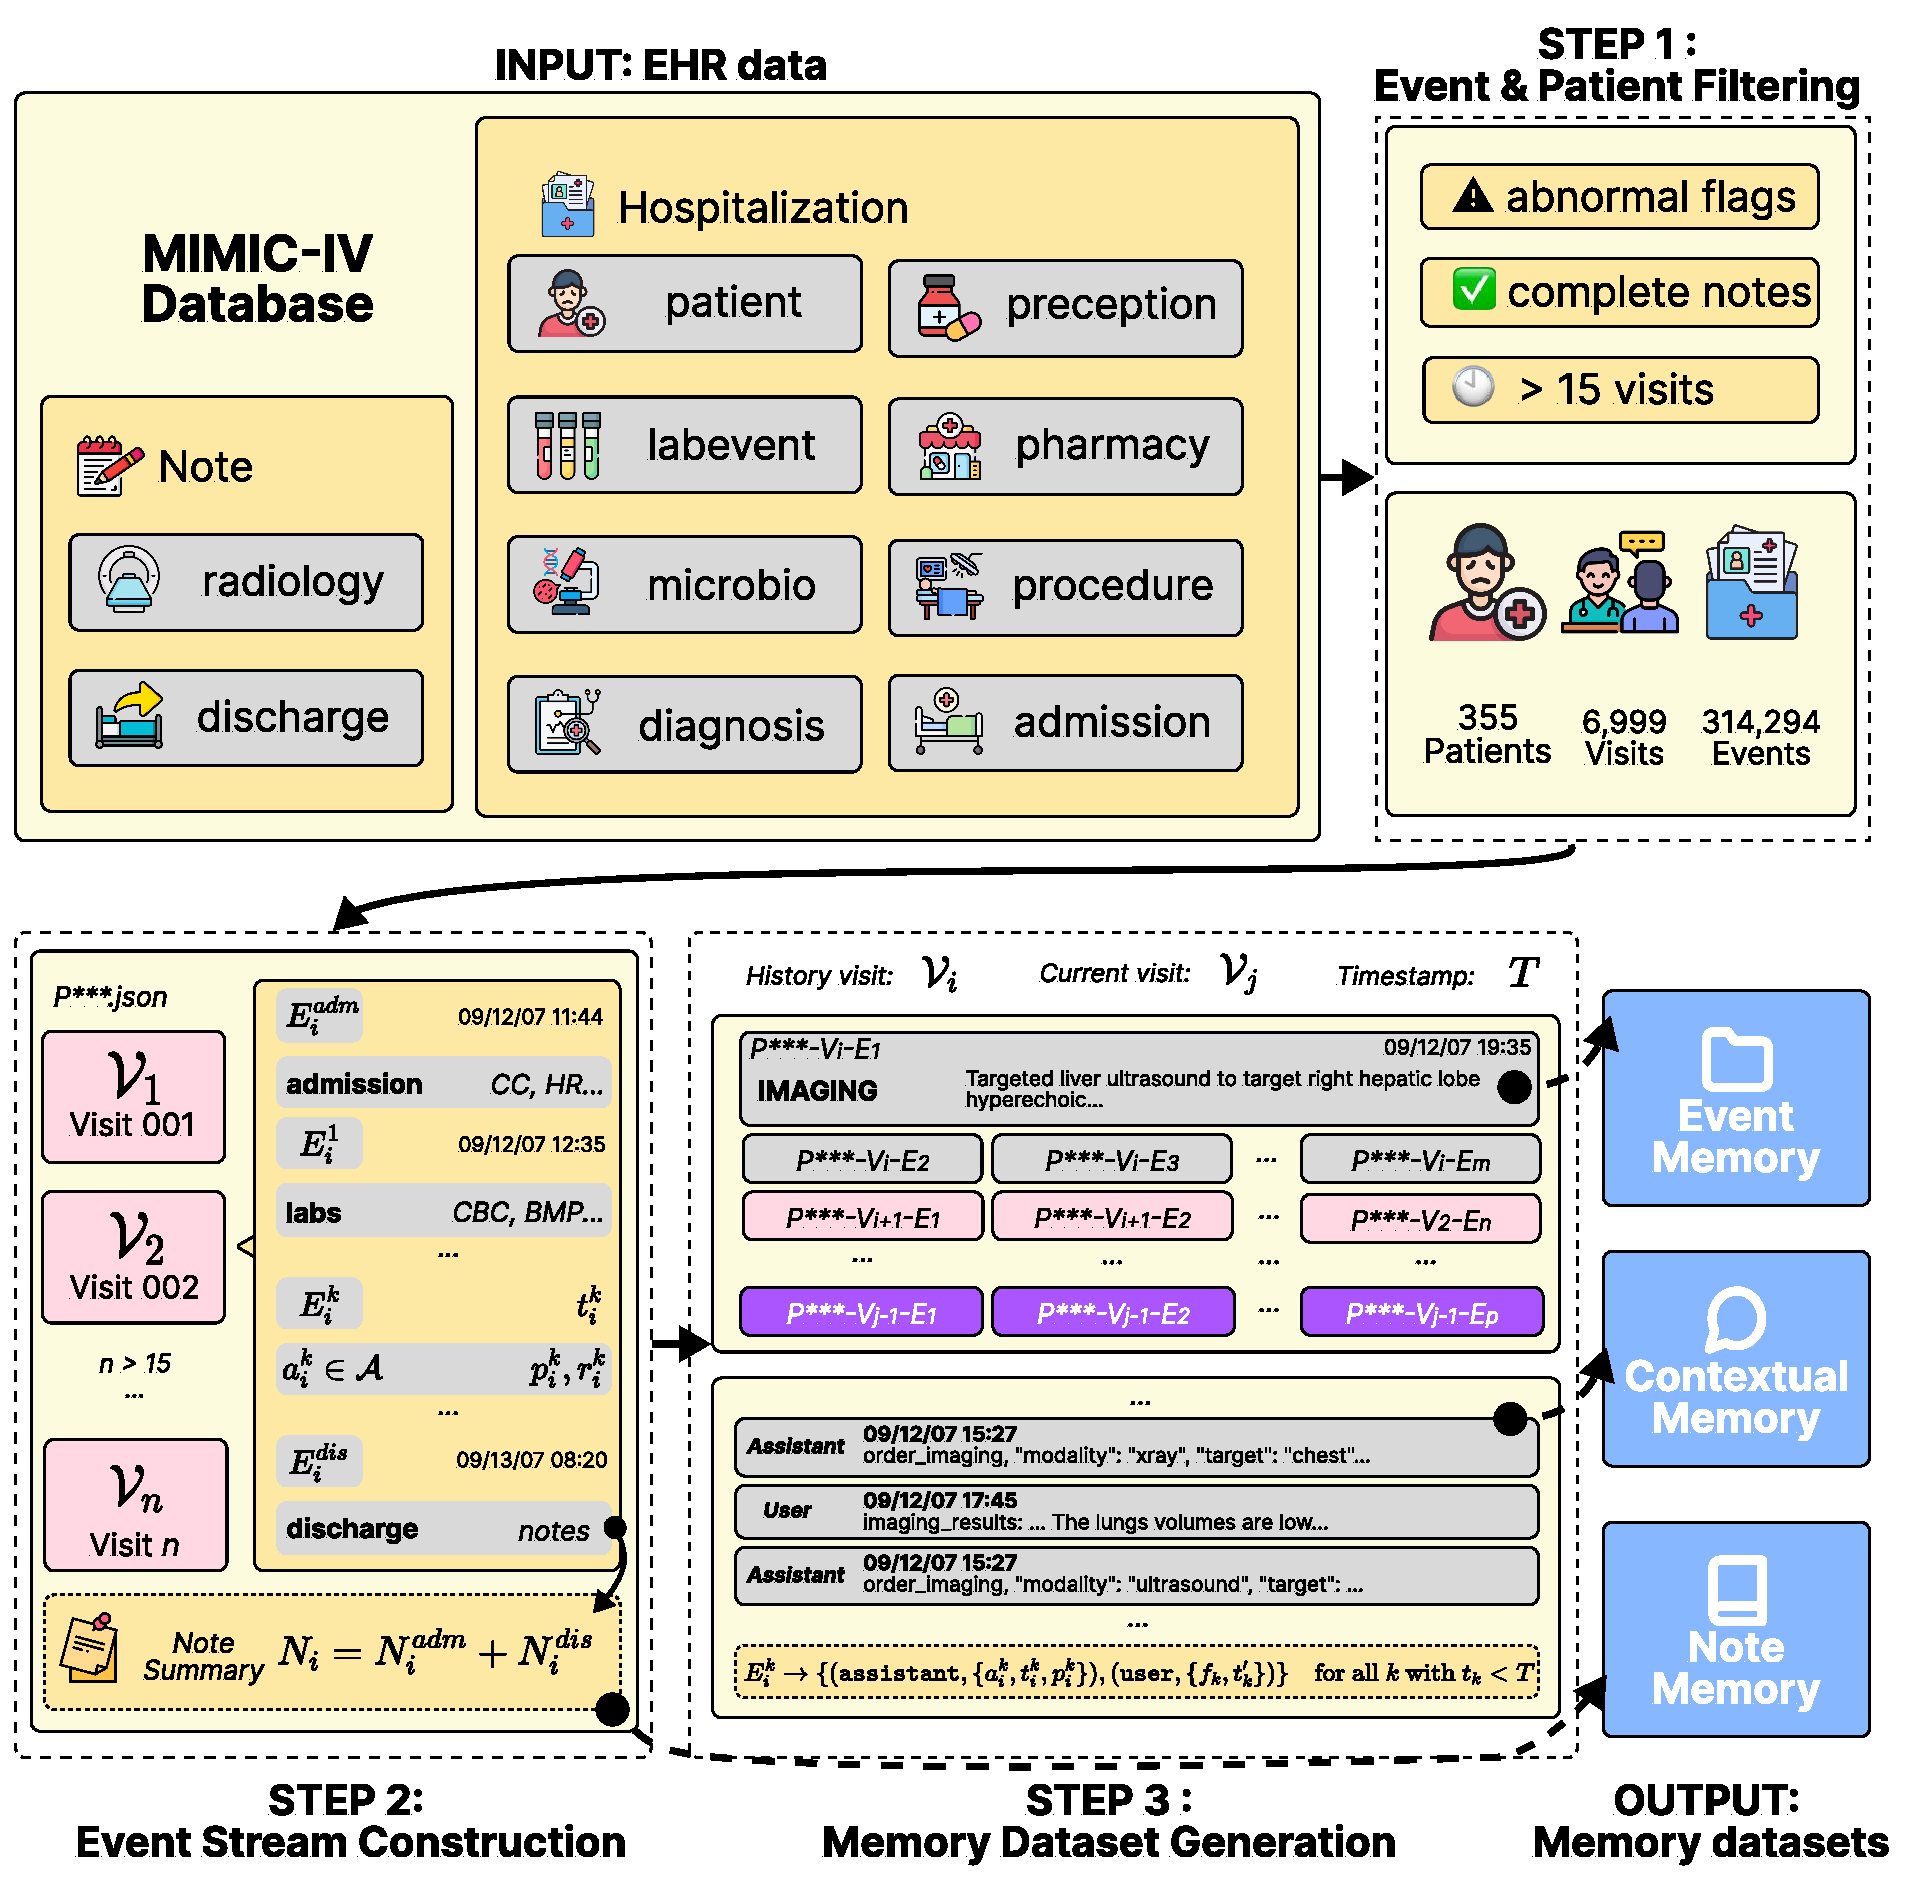
\includegraphics[width=\textwidth]{images/dataset_pipeline.pdf}
    \caption{Overview of the EHR data processing pipeline.}
    \label{fig:pipeline}
\end{figure}

LongMedBench is constructed from MIMIC-IV v3.1 \cite{PhysioNet-mimiciv-3.1}, a publicly available de-identified database containing comprehensive clinical data for over 100,000 patients at Beth Israel Deaconess Medical Center (2008--2022). To convert this database into an interactive agent-compatible environment, we design a three-stage pipeline (Figure~\ref{fig:pipeline}).


\subsection{Data Preprocessing \& Event Filtering}

\paragraph{Event-Level Filtering.} All structured clinical events are extracted from the \texttt{hosp} module, including laboratory measurements, microbiology cultures, medication prescriptions, pharmacy bills, diagnoses and procedures. Among these, we retain only laboratory results flagged as abnormal; normal lab values are excluded. Other events are retained in full. The rationale for this selective filtering strategy is discussed in Chapter~3.

From the \texttt{admissions} table, we decompose each hospitalization into two boundary events. The admission event captures the patient's demographics, chief complaint, and initial physical examination findings at intake. The discharge eventcaptures the discharge narrative and the final diagnoses recorded in \texttt{diagnoses\_icd}. 

\paragraph{Patient-Level Preprocessing.} We require each hospitalization to have a complete discharge summary from the \texttt{note} module whose timestamp aligns with the corresponding admission record in \texttt{hosp/admissions}; visits lacking a matched discharge note are excluded. From the remaining visits, we select patients with at least 15 recorded hospitalizations. The rationale for these filtering decisions is discussed in Chapter~3. 

\paragraph{Note Preprocessing.} Radiology reports are converted to structured imaging events via regular expression parsing: the modality \textit{(e.g., CT, X-ray, MRI)} and body region \textit{(e.g., chest, abdomen)} are extracted as the action type and parameter, respectively, while the full report text is retained as the observation result. Discharge notes $N_i$ are decomposed into admission information $N_i^{adm}$ and discharge information $N_i^{dis}$, then attached to the corresponding admission or discharge events. Both summaries are preserved in narrative format for use in Note Memory (Section~\ref{sec:notemem}) and ground-truth extraction. 

\paragraph{Resulting Cohort.} The filtered dataset comprises 355 patients with 6,999 inpatient visits. Mean visits per patient: 19.72 (median = 18.00, SD = 5.72). Mean medical events per visit: 44.91 (median = 25.00, SD = 70.32). The distribution of data is shown in Figure~\ref{fig:visit_distribution}. This dense multi-session structure challenges models on cross-visit memory retention and temporal reasoning.

\begin{figure}[ht]
    \centering
    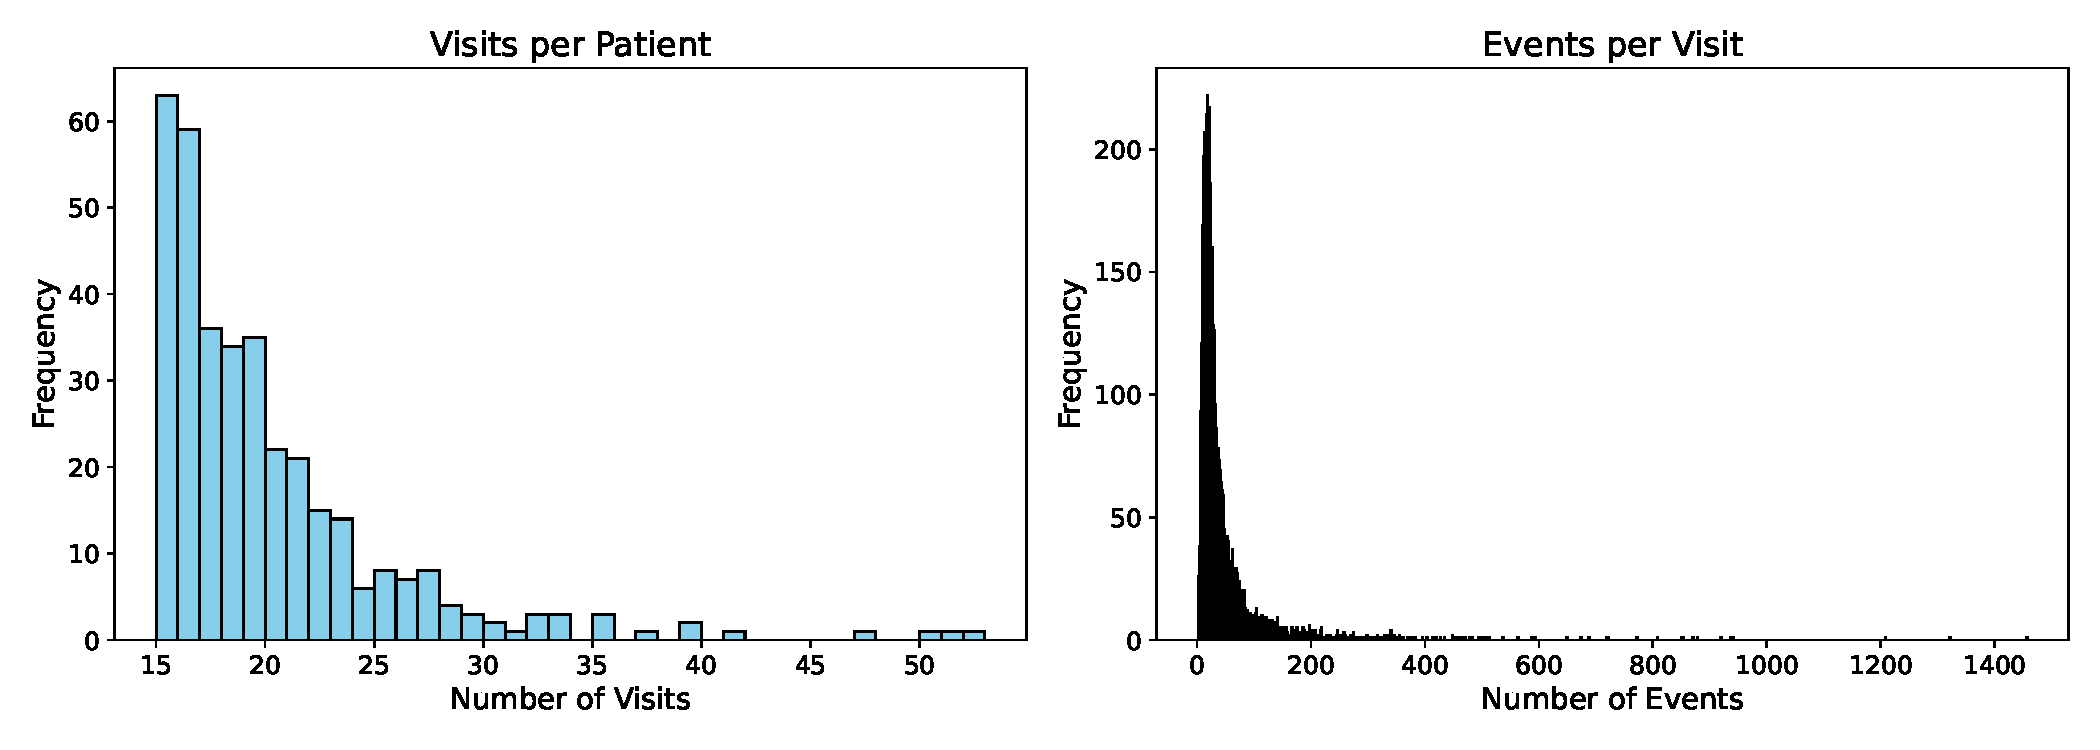
\includegraphics[width=\textwidth]{images/visit_distribution.pdf}
    \caption{Distribution of visits per patient in the filtered cohort.}
    \label{fig:visit_distribution}
\end{figure}

\subsection{Event Stream Construction}

We transform filtered records into a unified, time-ordered event stream for each patient. A medical event is any discrete clinical occurrence extracted from the structured hospitalization data. Formally, the $k_\text{th}$ event in $\mathcal{V}_i$ is $E^k_i := \{a^k_i, t^k_i, p^k_i, o^k_i\}$, where $a^k_i$ is the action type from the clinical action space $\mathcal{A}$, \textit{including imaging, lab tests, medication, etc.}, $t^k_i$ is the timestamp, $p^k_i$ is the action parameter \textit{(e.g., CT, X-ray, etc. for imaging)}, and $o^k_i$ is the observation result \textit{(e.g., a radiology report)}.

We define a visit as the period spanning from an admission event $E^{adm}_i$ to the corresponding discharge event $E^{dis}_i$. All other structured events occurring between these two timestamps are collected and ordered chronologically. Formally, each visit $\mathcal{V}_i$ can be represented as $\mathcal{V}_i = \{E^{adm}_i, E^1_i, E^2_i, \dots, E^m_i, E^{dis}_i\}$. The complete patient stream can therefore be denoted as $\mathcal{S_P} = \{\mathcal{V}_1, \mathcal{V}_2, \dots, \mathcal{V}_n\}$, where $n$ is the total number of visits.

\section{Three-Tier Memory Architecture}
\label{sec:memory}

To provide the agents with controlled provision of historical information, we define a three-tier memory architecture that systematically varies the granularity of historical information. Given the earliest historical visit $\mathcal{V}_i$, the current visit $\mathcal{V}_j$, and the current timestamp $T$, the agent's memory access is strictly bounded to prevent event leakage.

\subsection{Note Memory}
\label{sec:notemem}

$\mathcal{M}^{(i,j)}_N := \{N_i, N_{i+1}, \dots, N_{j-1}\}$, which contains continuous visit-level discharge summaries from $\mathcal{V}_i$ to $\mathcal{V}_{j-1}$. Note Memory is compact and preserves clinical narrative structure, emphasizing the global trajectory, but discards fine-grained temporal and event-level details.

\subsection{Event Memory}
\label{sec:eventmem}

$\mathcal{M}^{(i,j)}_E := \bigcup_{k=i}^{j-1} \mathcal{V}_k$, which contains all clinical events from $\mathcal{V}_i$ to $\mathcal{V}_{j-1}$. Events are flattened into a single chronological sequence, discarding visit-level boundaries and forming a unified trajectory. Event Memory is information-complete, and its volume creates a natural stress test for both long-context capabilities and retrieval strategies.

\subsection{Context Memory}
\label{sec:contextmem}

$\mathcal{M}_C^{(j,T)} := \{(r_0, m_0), (r_1, m_1), \dots, (r_P, m_P)\}$, where $r_k$ and $m_k$ denote the dialog role (\texttt{assistant} or \texttt{user}) and message content, respectively. Rewritten by LLM, any event $E_j^k$ in $\mathcal{V}_j$ with timestamp $t_j^k < T$ is transformed into a conversation trajectory between the agent and the clinical environment, simulating the agent's instant interaction state up to the decision point. 

Context Memory represents the baseline information always available to the agent. Historical memory ($\mathcal{M}^{(i,j)}_N$ or $\mathcal{M}^{(i,j)}_E$) is the experimental variable, enabling isolation of the marginal contribution of history beyond the immediate clinical context.

\section{Long-Horizon Decision-Making Task}
\label{sec:task}

\subsection{Task Formulation}

For a sampled ground-truth event $E_i^{GT}$ in the current visit $\mathcal{V}_i$ with timestamp $t_i^{GT}$, the working context is defined as $S=\mathcal{M}_C^{(i,t_i^{GT})}$, containing all interaction history available before the target event. The long-horizon memory is denoted as $M=\mathcal{M}^{(1,n)}_E$ or $M=\mathcal{M}^{(1,n)}_N$, depending on whether Event Memory or Note Memory is injected. At inference time, the agent receives $S$, an instructional prompt, $M$, and a multiple-choice query $Q$, then outputs an answer $\hat{y}$. The three subtasks are defined as follows:
\begin{itemize}
    \item   \textbf{Next Action Prediction} asks the agent to predict the future event action type $a_i^{GT}$ from the clinical action space $\mathcal{A}$.
    \item   \textbf{Argument Prediction} asks the agent to predict the target event argument $p_i^{GT}$, such as which laboratory panels or imaging modality are most appropriate.
    \item   \textbf{Discharge Decision} asks whether the patient should be discharged within $6$ hours, yielding a binary Yes/No decision.
\end{itemize}

\begin{figure}
    \centering
    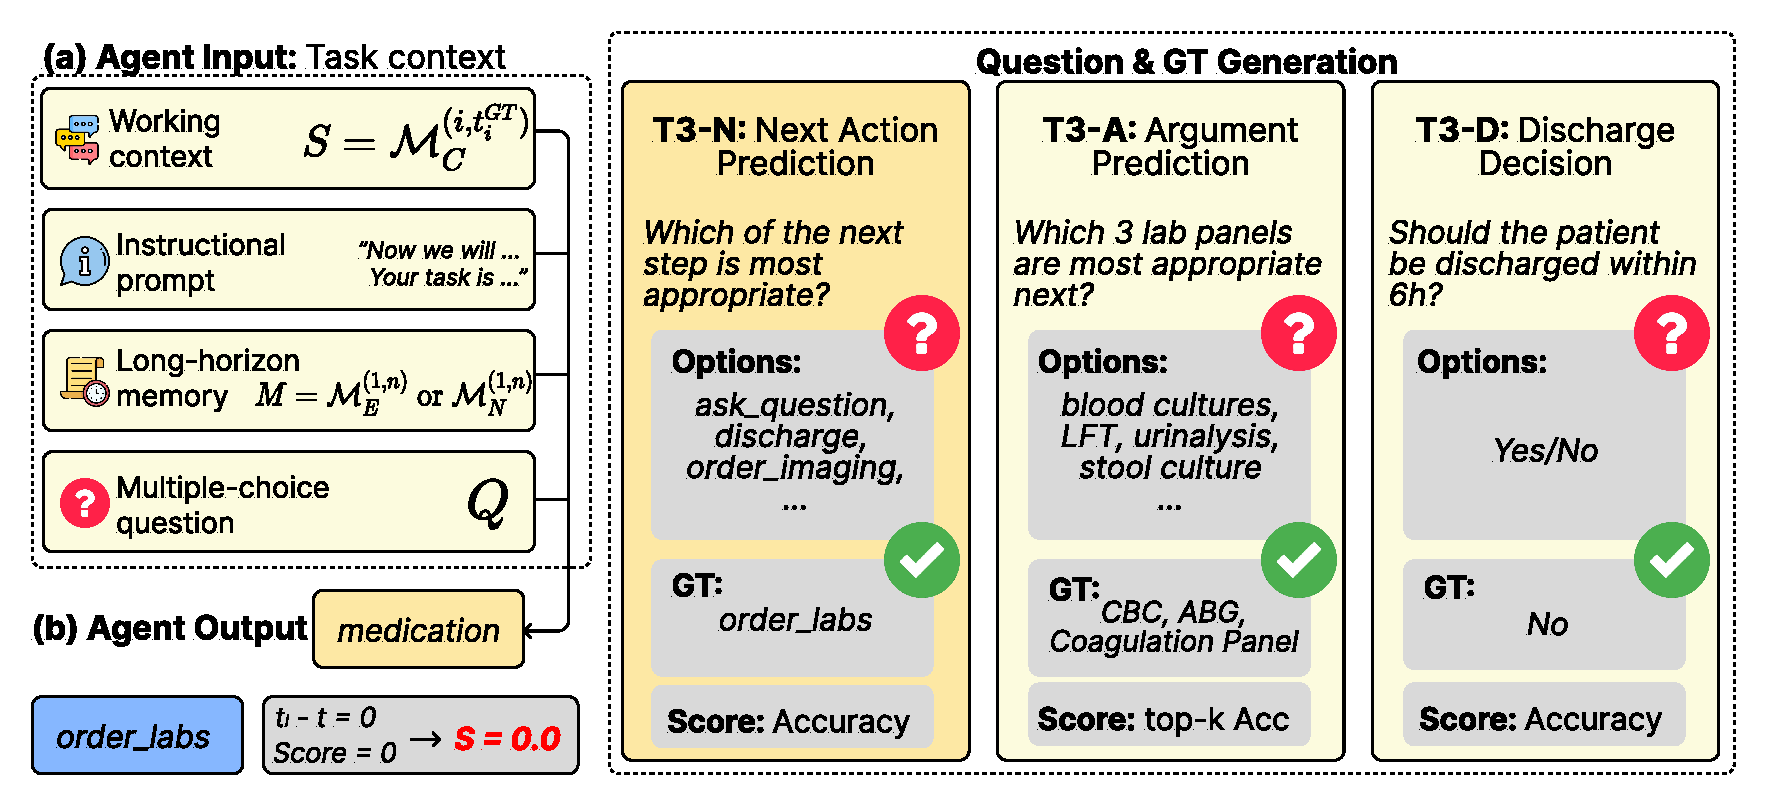
\includegraphics[width=\textwidth]{images/decision_making.pdf}
    \caption{Illustration of the long-horizon decision-making task.}
    \label{fig:decision_task}
\end{figure}

\subsection{Evaluation Metrics}

Next Action Prediction and Discharge Decision are evaluated by classification accuracy, while Argument Prediction is evaluated by top-$k$ accuracy because multiple arguments may be clinically appropriate. For Next Action Prediction and Argument Prediction, LongMedBench additionally applies a time-decay scoring mechanism to avoid over-penalizing decisions whose equivalent ground-truth action occurs shortly after the sampled timestamp. Let
\[
\mathcal{E}_{24h}=\{E_i^k \mid t_i^k\in[t_i^{GT},t_i^{GT}+24\mathrm{h}]\}.
\]
The score is
\[
S=\max_{E_i^k\in\mathcal{E}_{24h}}
\exp\{-\lambda(t_i^k-t_i^{GT})\}\cdot\operatorname{Score}(y_i^k,\hat{y}),
\quad
\lambda=\frac{\ln(100)}{24},
\]
where the decay factor decreases from $1.0$ at the target timestamp to $0.01$ after $24$ hours, $\operatorname{Score}(\cdot)$ is classification accuracy for Next Action Prediction and top-$k$ accuracy for Argument Prediction. Discharge Decision is evaluated directly as binary classification accuracy.

\section{Experimental Setup}
\label{sec:expsetup}

\subsection{Models}

We evaluate three state-of-the-art LLMs: GPT-5-mini, DeepSeek-v3.2 (with and without reasoning mode), and Qwen-Turbo. All are evaluated through their respective APIs with standardized prompts and default model configurations.

\subsection{Agent Architectures}

Given the fixed memory modules $\{\mathcal{M}^{(i,j)}_N, \mathcal{M}^{(i,j)}_E, \mathcal{M}_C^{(j,T)}\}$, three strategies control how historical memory is provided to the agent: \textbf{ (1) Naive Long-Context (Baseline).} $\mathcal{M}^{(i,j)}_N$ or $\mathcal{M}^{(i,j)}_E$ is provided in full within the model's context window alongside $\mathcal{M}_C^{(j,T)}$, testing native long-context attention without external retrieval assistance. \textbf{ (2) RAG.} $\mathcal{M}^{(i,j)}_N$ or $\mathcal{M}^{(i,j)}_E$ is externally indexed. At decision time, $\mathcal{M}_C^{(j,T)}$ serves as the retrieval query; top-$k$ relevant chunks are retrieved and concatenated with the context. This tests whether selective retrieval overcomes lost-in-the-middle effects. \textbf{(3) Agent Memory System.} We integrate the Mem0 framework \cite{mem0_reference}, providing a persistent, evolvable memory store to the agent. The agent can add, search, and update memory across a patient's trajectory, actively managing what is stored and retrieved. This tests whether agentic memory management outperforms passive retrieval.

\subsection{Experimental Conditions}

We design a factorial ablation varying four factors:

\begin{enumerate}
    \item \textbf{Memory Granularity:} Note Memory vs.\ Event Memory.
    \item \textbf{Provision Strategy:} Naive Long-Context vs.\ RAG vs.\ Mem0.
    \item \textbf{Historical Depth ($n$):} Number of injected historical visits: $n \in \{0, 1, 2, 3, \infty\}$. $n=0$ provides Context Memory $\mathcal{M}_C^{(j,T)}$ only (no history) as baseline.
    \item \textbf{Reasoning Mode:} Standard vs.\ chain-of-thought (DeepSeek-v3.2 only).
\end{enumerate}

Qwen-Turbo serves as the primary ablation vehicle; key conditions are replicated on GPT-5-mini and DeepSeek-v3.2 for cross-model validation.

\section{Results and Analysis}
\label{sec:results}

\subsection{Overall Decision-Making Performance Across Subtasks}

Table~\ref{tab:decision_overall} summarizes long-horizon decision-making performance under the naive long-context setting. We report all three decision-making subtasks rather than treating Discharge Decision as the entire benchmark. Across models, Discharge Decision is consistently easier than Next Action Prediction, while Argument Prediction falls between them. This separation is important: high discharge-decision accuracy does not imply strong action planning or argument selection.

\begin{table}[!h]
    \centering
    \caption{Long-context LLM performance on long-horizon decision-making. Argument evaluates event argument prediction, Discharge evaluates six-hour discharge decision, and Action evaluates next action-type prediction.}
    \label{tab:decision_overall}
    {\fontsize{8}{9.2}\selectfont
    \setlength{\tabcolsep}{2pt}
    \renewcommand{\arraystretch}{1.05}
    \begin{tabular*}{\textwidth}{l@{\extracolsep{\fill}}cccccccc}
        \toprule
        & \multicolumn{4}{c}{\textbf{Note Memory}} & \multicolumn{4}{c}{\textbf{Event Memory}} \\
        \cmidrule(lr){2-5}\cmidrule(lr){6-9}
        \textbf{Model} & \textbf{Argument} & \textbf{Discharge} & \textbf{Action} & \textbf{Avg} & \textbf{Argument} & \textbf{Discharge} & \textbf{Action} & \textbf{Avg} \\
        \midrule
        Qwen-Turbo & 0.475 & 0.604 & 0.309 & 0.434 & 0.494 & 0.604 & 0.309 & 0.420 \\
        DeepSeek-v3.2 & 0.478 & 0.607 & 0.278 & 0.422 & 0.493 & 0.607 & 0.304 & 0.439 \\
        GPT-5-mini & 0.478 & 0.625 & 0.324 & 0.445 & 0.494 & 0.607 & 0.335 & 0.452 \\
        DeepSeek-v3.2-thinking & 0.471 & 0.578 & 0.294 & 0.420 & 0.466 & 0.593 & 0.290 & 0.419 \\
        \bottomrule
    \end{tabular*}}
\end{table}

\subsection{Subtask-Level Patterns}

The most visible pattern is that Discharge Decision should not be interpreted as the whole decision-making task. It reaches approximately 0.58--0.63 because it is a binary discharge decision, whereas Next Action Prediction remains around 0.28--0.34 because selecting the next action type requires finer-grained clinical planning. Argument Prediction lies in the middle, reflecting the difficulty of selecting appropriate event arguments such as laboratory panels or imaging targets. Event Memory slightly improves Argument Prediction in most models, suggesting that fine-grained historical events help parameter selection, but the gains do not consistently translate into higher average decision-making performance.

\subsection{Memory Ablations: Visit Injection and Retrieval Architectures}

Table~\ref{tab:decision_ablation} reports the Qwen-Turbo ablation used to test historical depth and memory-augmentation strategies. The $n=0$ setting provides only Context Memory $\mathcal{M}_C^{(j,T)}$ and no injected historical memory. Increasing the number of injected visits does not produce monotonic gains, and retrieval-based architectures remain close to or below the naive baseline.

\begin{table}[!h]
    \centering
    \caption{Ablation study on long-horizon decision-making using Qwen-Turbo. The left block varies injected visit history; the right block compares retrieval/memory architectures.}
    \label{tab:decision_ablation}
    {\fontsize{8}{9.2}\selectfont
    \setlength{\tabcolsep}{4pt}
    \renewcommand{\arraystretch}{1.05}
    \begin{tabular*}{\textwidth}{ll@{\extracolsep{\fill}}cccc}
        \toprule
        \textbf{Setting} & \textbf{Memory/Arch} & \textbf{Argument} & \textbf{Discharge} & \textbf{Action} & \textbf{Avg} \\
        \midrule
        \multicolumn{6}{l}{\textbf{Visit Injection}} \\
        $n=0$ & -- & 0.49 & 0.61 & 0.32 & 0.45 \\
        $n=2$ & Event & 0.49 & 0.60 & 0.32 & 0.44 \\
        $n=5$ & Event & 0.48 & 0.60 & 0.31 & 0.43 \\
        $n=2$ & Note & 0.48 & 0.60 & 0.32 & 0.44 \\
        $n=5$ & Note & 0.48 & 0.60 & 0.32 & 0.44 \\
        \midrule
        \multicolumn{6}{l}{\textbf{Memory Architecture}} \\
        RAG & Event & 0.45 & 0.51 & 0.29 & 0.40 \\
        Mem0 & Event & 0.47 & 0.62 & 0.31 & 0.44 \\
        RAG & Note & 0.48 & 0.60 & 0.31 & 0.44 \\
        Mem0 & Note & 0.46 & 0.56 & 0.29 & 0.41 \\
        \bottomrule
    \end{tabular*}}
\end{table}

\textbf{Finding.} The ablation results revise the earlier interpretation: the negative result is not specific to Discharge Decision, but spans the broader decision-making suite. Even when historical information is made available through longer visit injection, RAG, or Mem0, models do not systematically improve on Argument Prediction, Discharge Decision, or Next Action Prediction. The $n=0$ baseline remains competitive, indicating that agents rely heavily on immediate context and struggle to convert retrieved history into better decisions.

\subsection{Chain-of-Thought Reasoning}

Explicit chain-of-thought reasoning does not improve decision-making performance for DeepSeek-v3.2. Under Event Memory, the average score drops from 0.439 to 0.419, and Discharge Decision decreases from 0.607 to 0.593. This suggests that reasoning mode may make the model more conservative or distract it from committing to the multiple-choice decision, especially when the task requires selecting an actionable next step rather than explaining uncertainty.

\subsection{Summary of Findings}

The experimental results converge on a refined narrative: (1) decision-making remains challenging, especially for Next Action Prediction; (2) Discharge Decision is easier and should not be used as a proxy for the entire decision-making benchmark; (3) Event Memory can modestly improve Argument Prediction but does not reliably improve average decision-making performance; (4) historical visit injection, RAG, and Mem0 do not provide systematic gains over the immediate-context baseline; and (5) chain-of-thought reasoning can degrade performance through increased conservatism. These findings collectively reveal a retrieval-reasoning gap whose implications we explore in Chapter~3.

\subsection{Qualitative Case Studies}

To ground the quantitative results in concrete agent behaviors, we inspect representative decision instances from the evaluation set. The following cases illustrate how memory architecture and memory type shape agent decisions at the level of individual queries.

\paragraph{Historical memory can change answers---sometimes for the worse.}
In a Next Action Prediction instance for a chemotherapy patient (Patient~3, Visit~16), the ground-truth next action is \texttt{medication}. With no injected history ($n=0$), the agent correctly selects \texttt{medication}, reasoning that furosemide is needed to manage fluid overload during chemotherapy. At $n=2$, the same correct answer is produced. However, at $n=5$, the agent switches to \texttt{order\_labs}, now reasoning that ``the patient is undergoing R-ICE chemotherapy and has abnormal lab results, indicating the need for further laboratory testing.'' Five historical visits introduce enough distracting context to overrule the initially correct decision. This non-monotonic pattern---correct at moderate history, wrong at longer history---mirrors the aggregate ablation results and suggests that longer context can dilute rather than strengthen clinical judgment.

\paragraph{Retrieved history can mislead when it mimics the current presentation.}
In an Argument Prediction instance (Patient~1, Visit~20), the agent must select the most appropriate next imaging study for a patient with bilateral lower-extremity edema. The long-context baseline correctly selects \texttt{XRAY abdomen}, reasoning that systemic conditions such as liver disease or heart failure warrant abdominal evaluation. The RAG-augmented agent selects \texttt{CT chest}, distracted by retrieved note text mentioning chest pain and a non-diagnostic chest X-ray. The Mem0-augmented agent selects \texttt{CT head}, focusing on a retrieved headache complaint from an earlier visit. Both retrieval-based agents are led astray by historical snippets that superficially match but are clinically irrelevant to the current presentation. This illustrates a concrete failure mode: when retrieval returns temporally nearby but causally unrelated events, the agent conflates them with the immediate clinical context.

\paragraph{Note Memory can misattribute retrieved content to the current visit.}
In another Next Action Prediction instance (Patient~1, Visit~20), the ground-truth action is \texttt{order\_labs}. The Mem0 agent correctly selects \texttt{order\_labs} under Event Memory, citing persistent electrolyte abnormalities and rising creatinine. Under Note Memory, however, the same agent switches to \texttt{medication}, justifying the choice with a positive stool culture for \textit{Salmonella} found in a retrieved discharge summary from a prior admission. The agent fails to distinguish a retrospective finding from a current clinical need, treating historical note content as actionable evidence for the present visit. This confusion is less likely under Event Memory, where explicit timestamps and structured fields make temporal provenance clearer.

\subsection{Discussion of Negative Results}

The finding that memory augmentation does not improve decision-making may appear discouraging, but it carries productive implications. First, it identifies a genuine capability gap that current architectures cannot bridge through scale or retrieval quality alone---the gap is architectural, not parametric. Second, it provides a clear target for future work: architectures that explicitly model the relationship between retrieved history and current decisions, rather than treating retrieval as an independent preprocessing step. Third, the qualitative cases reveal specific failure modes---context dilution at longer histories, distraction by superficially similar retrieved snippets, and temporal misattribution of note content---that are diagnosable and potentially addressable through memory designs that preserve temporal provenance and causal relevance.

The contrast with EHR-Bench \cite{2025_ehr_r1} is instructive. EHR-Bench demonstrated that LLMs can predict next clinical events from complete histories with non-trivial accuracy, but our agent-based setting reveals that this does not translate to interactive decision-making where history must be selectively retrieved and integrated. The two paradigms evaluate complementary but distinct capabilities---static prediction vs.\ interactive planning---and the gap between them highlights the importance of evaluation methodology in assessing clinical AI readiness.

\chapter{Discussion and Conclusion}

\section{Summary of Findings}

The experimental results presented in Chapter~2 yield five key findings:

\textbf{1. Decision-making remains challenging.} Across GPT-5-mini, DeepSeek-v3.2, and Qwen-Turbo, average decision-making performance remains around 0.42--0.45, with substantial variation across subtasks. The Discharge Decision is the easiest subtask (roughly 0.58--0.63), while Next Action Prediction remains much lower (roughly 0.28--0.34). This gap shows that binary discharge judgment should not be treated as a proxy for full clinical decision-making ability.

\textbf{2. Memory granularity matters modestly.} Structured Event Memory slightly outperforms Note Memory in most conditions, but the effect is small relative to the overall performance ceiling. For proactive clinical planning, immediate context dominates.

\textbf{3. Memory augmentation does not improve decision-making.} This is the central finding. Neither RAG nor Mem0 provides significant improvement over the naive long-context baseline. In some conditions, augmentation slightly degrades performance.

\textbf{4. Immediate context dominates historical context.} The $n=0$ baseline ($\mathcal{M}_C^{(j,T)}$ only, no history) achieves accuracy comparable to full-history conditions. Adding historical visits does not monotonically improve decisions.

\textbf{5. Chain-of-thought can degrade performance.} For DeepSeek-v3.2 under Event Memory, reasoning mode reduces average decision-making performance from 0.439 to 0.419 and Discharge Decision accuracy from 0.607 to 0.593, likely because explicit reasoning induces conservatism that penalizes decisive action under multiple-choice evaluation.

\section{The Retrieval-Reasoning Gap}

These findings collectively reveal a \textbf{retrieval-reasoning gap}: a disconnect between LLMs' ability to \emph{locate} relevant historical information and their ability to \emph{integrate} that information into proactive clinical planning. This explains why RAG and Mem0 fail: these architectures optimize retrieval quality, but for clinical decision-making, retrieval is not the bottleneck. The model can access relevant history (either in full context or via retrieval), but cannot effectively use it to inform decisions.

We hypothesize three contributing mechanisms. First, clinical reasoning requires causal, not associative, inference---determining whether a prior treatment was effective requires understanding why it was given and how the patient responded, not just retrieving that it occurred. Second, the signal-to-noise ratio in longitudinal EHR data is low: a patient's 900 events contain only a fraction relevant to any single decision, overwhelming attention mechanisms. Third, current LLM training data (web text, code, books) lacks the temporal-causal structure of clinical trajectories, creating a distribution shift.

\section{Implications}

\subsection{For Memory Architecture Design}

Current memory architectures (RAG, Mem0, MemGPT) operate on the assumption that better retrieval yields better performance. Our findings challenge this assumption for clinical decision-making. Future architectures should emphasize \emph{reasoning over retrieved information}: temporal attention mechanisms that encode causal relevance, graph-based representations that capture clinical relationships, and structured reasoning layers that bridge retrieval and decision.

\subsection{For Benchmark Design}

If decision-making performance is dominated by immediate context, benchmarks that primarily test retrieval may overestimate clinical readiness. We advocate for adversarial task design---constructing decision instances where history \emph{changes} the correct answer---to prevent models from succeeding through immediate-context heuristics alone. Additionally, distinguishing the subset of decisions where history genuinely matters from those driven by current presentation is critical for targeted evaluation.

\subsection{For Clinical AI Deployment}

The finding that immediate context dominates is not necessarily a weakness---in many clinical scenarios, the current presentation is indeed the most important determinant. The challenge lies in identifying decisions where ignoring history constitutes clinical error (e.g., prescribing a medication that previously caused an adverse reaction) and ensuring the agent has the architecture to recognize and act on such cases.

\section{Limitations}

\textbf{Data Scope.} LongMedBench is constructed from MIMIC-IV, a single-institution database. Clinical practice patterns and documentation conventions vary across institutions, and findings may not generalize without cross-institutional validation.

\textbf{Cohort Bias.} Several design decisions in our data pipeline shape the cohort composition. At the event level, we retain only laboratory results flagged as abnormal, following Hager et al.\ \cite{hager2024evaluation}, who demonstrated that presenting models with only abnormal lab values improved diagnostic performance in MIMIC-CDM by reducing noise from clinically uninformative normal results. This filtering makes the evaluation more clinically realistic---like human clinicians, the agent reasons from salient pathological signals---but may underrepresent the diagnostic challenge of distinguishing normal variation from true abnormality. At the patient level, we require each hospitalization to have a matched discharge note from the \texttt{note} module and select patients with $\ge 15$ hospitalizations. We chose this threshold after examining the trade-off between trajectory length and cohort size: lowering to $\ge 10$ visits yields trajectories too short to meaningfully evaluate cross-visit reasoning; raising to $\ge 20$ visits produces trajectories of over 20 steps but retains only approximately 100 patients, limiting statistical power. At $\ge 15$ visits, the resulting cohort of 355 patients compares favorably to sample sizes in other EHR-based agent benchmarks---MedAlign enrolled 276 patients \cite{2024_medalign} and DiReCT enrolled 511 patients \cite{wang2024direct}. Nevertheless, this threshold selects for high-acuity, chronic, multi-morbid patients---the population for whom longitudinal reasoning matters most---and findings may not generalize to lower-acuity settings or the broader patient base.

\textbf{Task Simplification.} The benchmark decomposes clinical decision-making into three multiple-choice subtasks: Next Action Prediction predicts the next event action type, Argument Prediction predicts the event argument, and Discharge Decision predicts six-hour discharge readiness. This decomposition improves diagnostic clarity but still simplifies real clinical decisions, which involve dosing, contraindication checking, patient preferences, resource availability, and guideline compliance not fully captured by our formulation.

\textbf{Question Discriminability.} Not all evaluation questions are equally informative. An analysis of model agreement reveals that the Discharge Decision subtask has extremely few discriminative instances: only 8 out of 448 sampled questions (~1.8\%) produce disagreement across model configurations; the vast majority yield unanimous scores of 1.0 because patients are simply too early or too late for discharge. This inflates apparent Discharge Decision accuracy and limits its diagnostic value for comparing architectures. The Next Action Prediction subtask, by contrast, has approximately 70\% discriminative questions, making it the most informative component of the decision-making benchmark.

\textbf{Evaluation Rigor.} Classification accuracy for Next Action Prediction and Discharge Decision and top-$k$ accuracy for Argument Prediction may penalize clinically reasonable alternatives. The time-decay mechanism partially addresses timing ambiguity for Next Action Prediction and Argument Prediction, but no automatic metric replaces clinical expert judgment. We recommend human clinician evaluation as a future validation step.

\textbf{Model Coverage.} Our evaluation covers three general-purpose LLMs. Models specifically trained for clinical tasks (e.g., EHR-R1, Med-PaLM) may exhibit different patterns not captured here.

\section{Future Work}

\textbf{Task Refinement.} Adversarial decision instances where history changes the correct answer would directly test temporal integration. Counterfactual evaluation---altering history and measuring decision sensitivity---would isolate causal effects.

\textbf{Memory Architecture Development.} Temporal graph memory, selective history summarization (compressing irrelevant while preserving salient information), and memory-aware fine-tuning on synthetic longitudinal trajectories are promising directions.

\textbf{Human Baseline.} A clinician evaluation study contextualizing both average decision-making performance (approximately 0.42--0.45) and subtask-specific performance would validate benchmark difficulty and enable calibrated assessment of model progress.

\textbf{Cross-Institutional Validation.} Extending the pipeline to eICU, HiRID \cite{2021_hirid_icu}, or STARR would test generalizability across institutions and patient populations.

\textbf{Multimodal Extension.} Incorporating medical imaging and physiological waveforms would increase clinical fidelity as vision-language and multimodal LLMs mature.

\textbf{Outcome Correlation.} Linking agent decisions to simulated patient outcomes (mortality, readmission, length of stay) would provide the ultimate validation of decision-making quality.

\section{Conclusion}

Clinical practice is inherently longitudinal---patients accumulate histories over years, and clinicians must integrate evidence across this temporal expanse. As LLMs move toward clinical deployment, their capacity for longitudinal reasoning becomes a critical benchmark.

This thesis presented the decision-making component of LongMedBench, investigating how contemporary LLMs use historical clinical information to inform proactive planning through a three-tier memory architecture and systematic ablation experiments. The central finding is that memory augmentation---the dominant paradigm for extending LLM capabilities---does not significantly improve longitudinal clinical decision-making. Decision accuracy depends primarily on immediate context, and historical information, however organized, contributes marginal additional value.

This finding clarifies the nature of the challenge. The bottleneck is not retrieval---finding the right facts---but integration---understanding how those facts collectively inform decisions. Closing this retrieval-reasoning gap requires architectures that go beyond retrieval to support structured reasoning over temporal clinical evidence. The path to clinically capable AI agents is longer than single-encounter benchmarks suggest, but by identifying where current approaches fall short, LongMedBench provides a platform for measuring and ultimately closing this gap.

\subsection{Relationship to the Broader LongMedBench Project}

While this thesis focuses on the Long-Horizon Decision-Making task, placing our findings in the context of the broader LongMedBench project reveals complementary insights. LongMedBench also includes a Factual QA task, which tests factual retrieval from long clinical histories, and a Temporal Reasoning task, which tests event and visit ordering. These tasks help separate retrieval, temporal reconstruction, and decision-making.

The contrast between these task suites sharpens our central finding: memory augmentation can help retrieval-oriented tasks, but it does not reliably improve decision-making across Next Action Prediction, Argument Prediction, and Discharge Decision subtasks. This dissociation confirms that the retrieval-reasoning gap is task-specific---it manifests when the agent must do more than locate facts, when it must convert longitudinal evidence into an actionable decision. This insight would not be visible from any single task suite; it emerges only from the systematic, multi-dimensional evaluation that LongMedBench provides.

\subsection{Practical Considerations for Reproducibility}

The MIMIC-IV data itself requires credentialed access through PhysioNet. To facilitate reproducibility and future extensions, we will release the data processing pipeline, task generation logic, and evaluation harness, if LongMedBench is admitted by MICCAI 2026. 

API-based model evaluation used default settings and fixed random seeds where applicable. Full prompt templates, including system prompts, memory formatting conventions, and decision queries, are documented in the released codebase to ensure exact replication.


% 使用bib方式插入参考文献，

\clearpage

\renewcommand{\bibname}{\xiaoyi\bf\vspace{5pt} References}
\addcontentsline{toc}{chapter}{References}
\bibliographystyle{gbt7714-numerical}
\singlespacing

\bibliography{ref}
\doublespacing


% 直接插入参考文献，
% \include{data/ref}

\centerline{\xiaoyi\bf Appendix}
\addcontentsline{toc}{chapter}{Appendix}

\section*{A. LongMedBench Pipeline and Artifact Card}
\addcontentsline{toc}{section}{A. LongMedBench Pipeline and Artifact Card}

This appendix documents the implementation pipeline used to construct the Long-Horizon Reasoning Task data and run agent evaluation. The project artifacts are hosted on the cloud server under \texttt{/data/lab/LongMedBench}. Following common supplementary-material practice in top AI conferences, the appendix separates reproducibility metadata, pipeline stages, prompting interfaces, and qualitative evidence rather than listing source filenames in prose.

\subsection*{A.1 Reproducibility Card}
\addcontentsline{toc}{subsection}{A.1 Reproducibility Card}

\begin{table}[!h]
    \centering
    \caption{Reproducibility card for the LongMedBench long-horizon reasoning pipeline.}
    \label{tab:appendix_artifact_card}
    {\fontsize{8}{9.2}\selectfont
    \setlength{\tabcolsep}{3pt}
    \renewcommand{\arraystretch}{1.15}
    \begin{tabular*}{\textwidth}{p{0.22\textwidth}@{\extracolsep{\fill}}p{0.70\textwidth}}
        \toprule
        \textbf{Item} & \textbf{Description} \\
        \midrule
        Cloud location & The codebase and generated artifacts are stored at \texttt{/data/lab/LongMedBench} on the project server. \\
        Data source & MIMIC-IV v3.1 supplies hospitalization records, structured clinical events, radiology reports, discharge summaries, and ICU chart events. \\
        Cohort rule & Patients are retained only when all admissions have matched discharge summaries and the longitudinal trajectory contains at least \texttt{MIN\_VISITS=15} hospitalizations. \\
        Benchmark scale & The current filtered cohort contains 355 patients and 6,999 inpatient visits, yielding dense multi-visit trajectories for long-horizon evaluation. \\
        Memory types & Note Memory summarizes prior visits, Event Memory preserves structured event streams, and Context Memory stores the current-visit interaction state before the decision point. \\
        Evaluation modes & Runs vary model family, historical-memory type, and memory provision strategy, including long-context prompting, retrieval augmentation, and agent-managed memory. \\
        \bottomrule
    \end{tabular*}}
\end{table}

\begin{table}[!h]
    \centering
    \caption{Pipeline stages for constructing LongMedBench long-horizon reasoning data.}
    \label{tab:appendix_pipeline_stages}
    {\fontsize{8}{9.2}\selectfont
    \setlength{\tabcolsep}{3pt}
    \renewcommand{\arraystretch}{1.15}
    \begin{tabular*}{\textwidth}{p{0.18\textwidth}@{\extracolsep{\fill}}p{0.28\textwidth}p{0.44\textwidth}}
        \toprule
        \textbf{Stage} & \textbf{Implementation layer} & \textbf{Output and role} \\
        \midrule
        Raw EHR ingestion & Structured hospitalization, note, and ICU modules & Admissions, diagnoses, medications, procedures, microbiology, radiology reports, discharge summaries, laboratory records, and ICU warning events provide the raw clinical substrate. \\
        Patient and event filtering & Cohort filtering and event normalization layer & Patients are retained under the longitudinal-trajectory rule above. Event preprocessing keeps abnormal ICU warning events and abnormal laboratory rows while preserving other structured event types downstream. \\
        Event stream construction & Visit-level event conversion layer & Each visit is converted into a chronologically ordered stream of typed clinical events, with admission and discharge boundaries, structured actions, timestamps, and event arguments. \\
        Memory dataset generation & Note slicing and context construction layer & Discharge summaries are sliced into admission and discharge fields, while structured events are serialized into context messages. These artifacts instantiate Note Memory, Event Memory, and Context Memory. \\
        Question generation & Reasoning-task construction layer & For each visit prefix, the benchmark constructs Next Action Prediction, Argument Prediction, and Discharge Decision questions from future events and discharge timing. \\
        \bottomrule
    \end{tabular*}}
\end{table}

The benchmark output follows a patient-centered artifact schema. Each retained patient has a static patient profile, a sequence of visit records, and generated decision questions indexed by visit and target timestamp. The organization is designed so that an evaluator can reconstruct, for any question, the current interaction context, the historical memory condition, the candidate options, the ground truth, and the model reply.

\subsection*{A.2 Agent Prompt and Memory Interfaces}
\addcontentsline{toc}{subsection}{A.2 Agent Prompt and Memory Interfaces}

The agent prompt exposes a small action space: \texttt{ask\_question}, \texttt{order\_labs}, \texttt{order\_microbiology}, \texttt{order\_imaging}, \texttt{perform\_procedure}, \texttt{medication}, and \texttt{discharge}. The memory labels map previous-visit discharge summaries to Note Memory, chronologically ordered previous-visit events to Event Memory, and completed current-visit dialogue state to Context Memory.

The direct question-answering system prompt is:
\begin{verbatim}
Now you are asked to answer agentic-desision questions without interacting with
the environment; in that case, you should answer based on the admission record
and NOT perform any environment actions.
Your message MUST be a JSON object with keys: {reason, answer}.
The answer should be a list containing only provided option from the question.
You should return the raw text of the option(s) as the answer, not the label
(e.g., "A", "B", ...). If multiple options are selected, include all of them
in the list. The reason should be a brief explanation based on the context and
admission history.
\end{verbatim}
For interactive use, the companion action prompt requires a JSON object with \texttt{reason}, \texttt{action}, and \texttt{args}; for benchmark question answering, the agent must not call environment actions and must instead return \texttt{reason} and \texttt{answer}. This ReAct-inspired, rationale-before-decision interface makes the model state an explicit reason before selecting the answer, while preventing it from inventing new observations and still allowing it to use the serialized admission record and selected historical memory.

\subsection*{A.3 Medical Event to Context Memory Conversion}
\addcontentsline{toc}{subsection}{A.3 Medical Event to Context Memory Conversion}

Context Memory converts a medical event into a dialogue-style trace between the agent and the clinical environment. The conversion uses the action type as the assistant-side decision, the structured argument as the action arguments, and the observation text as the environment-side response. Timestamps are retained so that the resulting context can be truncated strictly before the target event.

The prompt used for this conversion can be summarized as follows:
\begin{verbatim}
You are converting an electronic health record event into an interaction memory
for a medical decision-making agent.

Input:
- event_type: one of ask_question, order_labs, order_microbiology,
  order_imaging, perform_procedure, medication, discharge
- timestamp: the clinical event time
- arguments: structured event arguments, such as medication name, lab panel,
  imaging modality, or procedure name
- observation: the clinical result, report text, or environment feedback

Output a JSON array of dialogue messages. Use the assistant role for the action
selected by the agent and the environment role for the observed result. Preserve
the timestamp, do not infer new clinical facts, and keep the wording faithful to
the input event.

Expected output schema:
[
  {
    "role": "assistant",
    "timestamp": "<event timestamp>",
    "action": "<event_type>",
    "args": { ... }
  },
  {
    "role": "environment",
    "timestamp": "<event timestamp>",
    "content": "<observation>"
  }
]
\end{verbatim}

The conversion process has four steps: first, normalize the event into the benchmark action space; second, serialize the action arguments without adding clinical interpretation; third, attach the observation as an environment message; and fourth, sort all messages by timestamp before sampling the decision point. This design makes Context Memory an interaction history rather than an additional historical-memory condition.

\subsection*{A.4 Question Formats and Evaluation Protocol}
\addcontentsline{toc}{subsection}{A.4 Question Formats and Evaluation Protocol}

The Long-Horizon Reasoning Task is decomposed into three question formats whose final outputs are clinical actions, arguments, or discharge decisions:

\begin{itemize}
    \item \textbf{Next Action Prediction.} The question stem is ``Which of the next step is most appropriate?'' Options are sampled from the seven-action space above, and the ground truth is the action type of the next clinical event.
    \item \textbf{Argument Prediction.} The question asks for the argument of the next action, such as ``Which 2 medications are most appropriate next?'' or which imaging study is most appropriate. The ground truth is collected from matching future events in a 24-hour window.
    \item \textbf{Discharge Decision.} The question is a binary Yes/No decision asking whether the patient should be discharged within 6 hours. Unlike argument prediction, this subtask does not use the 24-hour decay window.
\end{itemize}

For future-event argument questions, the evaluator collects events in \((t,t+24h]\) and assigns an exponential decay weight:
\[
    \lambda = \frac{\ln(100)}{24}, \qquad w(\Delta t)=\exp(-\lambda \max(0,\Delta t)),
\]
so an event at the current time has weight 1.0 and an event 24 hours later has weight 0.01.

The expected model output is a JSON object:
\begin{verbatim}
{"reason": "The patient has abnormal lab results...", "answer": ["order_labs"]}
\end{verbatim}

The evaluator first parses the model reply as JSON. It accepts a plain JSON string or a fenced \texttt{json} block, extracts \texttt{reason} and \texttt{answer}, and normalizes the answer into a nonempty list of stripped strings. The weighted accuracy function then handles three ground-truth types:

\begin{enumerate}
    \item If the ground truth is a string, the prediction receives 1.0 when the string appears in the predicted list and 0.0 otherwise.
    \item If the ground truth is a dictionary from option to weight, the score is the clipped sum of weights for matched predicted options.
    \item If the ground truth is an unweighted list, the score is the fraction of ground-truth options recovered by the predicted set.
\end{enumerate}

The reported runs include Qwen-Turbo, DeepSeek-v3.2, and GPT-5-mini, with Note Memory and Event Memory supplied through long-context prompting, retrieval augmentation, or Mem0-style memory. A separate agreement analysis filters out unanimous questions to assess discriminability. This analysis shows that Discharge Decision has only 8 discriminative cases out of 448 sampled questions (about 1.8\%), while Next Action Prediction is substantially more discriminative. This finding motivates interpreting binary discharge accuracy cautiously and emphasizing subtask-level reporting.

\subsection*{A.5 Qualitative Case Studies and Original Interaction JSON}
\addcontentsline{toc}{subsection}{A.5 Qualitative Case Studies and Original Interaction JSON}

To ground the quantitative results in concrete agent behaviors, we inspect representative reasoning instances from the evaluation set. The cases show three recurring failure modes. First, historical memory can change answers for the worse: in a Next Action Prediction instance for a chemotherapy patient (Patient~3, Visit~16), the agent correctly selects \texttt{medication} with no injected history and with two previous visits, but switches to \texttt{order\_labs} when five visits are injected. Second, retrieved history can mislead when it mimics the current presentation: in an Argument Prediction instance for a patient with bilateral lower-extremity edema, retrieval-based agents are distracted by prior chest pain or headache snippets and select irrelevant imaging. Third, Note Memory can misattribute retrieved content to the current visit, treating a retrospective finding as present-time actionable evidence.

\paragraph{Original interaction trace.}
The following compact JSON excerpt is taken from the original remote artifacts. It preserves the dialogue/action structure while omitting long clinical note text. The trace shows a context in which the agent has just ordered Doppler imaging, receives a limited addendum, and then answers \texttt{ask\_question} even though the original EHR event used as ground truth is \texttt{order\_imaging}.
\begin{verbatim}
{
  "memory_type": "event",
  "visit_id": "P000001-V12",
  "t_index": 2,
  "timestamp": "2121-12-16 19:10:00",
  "question": "Which of the next step is most appropriate?",
  "ground_truth": {"order_imaging": 1.0},
  "context_excerpt": [
    {
      "role": "assistant",
      "timestamp": "2121-12-16 19:10:00",
      "action": "order_imaging",
      "args": {
        "modality": "doppler",
        "target": "free text body part"
      }
    },
    {
      "role": "environment",
      "timestamp": "2121-12-16 19:10:00",
      "content_excerpt": [
        "Addendum:",
        "A limited Color Doppler and Spectral Analysis Study was also",
        "performed."
      ]
    }
  ],
  "reply": {
    "reason": [
      "The Doppler study report is incomplete/unclear",
      "and only notes that a limited Doppler study was performed.",
      "It is appropriate to ask a clarifying question about",
      "the Doppler results before proceeding."
    ],
    "answer": ["ask_question"]
  },
  "score": 0.0,
  "source_files": {
    "context": [
      "tasks/agentic_decision/context/P000001",
      "P000001-V12.context.json"
    ],
    "question": [
      "tasks/agentic_decision/questions_generated",
      "P000001.jsonl:1"
    ],
    "prediction": [
      "agents/llm_agent/agentic_decision/results",
      "P000001.event.20260215-160939-a965d504.pred.jsonl:1"
    ]
  }
}
\end{verbatim}
Although the immediate context contains a recent imaging interaction, the model's explicit rationale treats the Doppler report as incomplete and selects \texttt{ask\_question}. The ground truth remains the next imaging action recorded in the original EHR event stream, so the prediction receives score 0.0.

\centerline{\xiaoyi\bf Author's Biography}
\addcontentsline{toc}{chapter}{Author's Biography}

\section*{1. Personal Information}

Name: Zihan Xu

Gender: Male

Date of Birth: February 27, 2004

Email: zihan1.22@intl.zju.edu.cn

\section*{2. Education}

September 2022--June 2026: Zhejiang University, ZJU-UIUC Institute, Bachelor of Engineering in Computer Engineering.

August 2024--May 2025: University of Illinois at Urbana-Champaign, exchange program in Computer Engineering.

\section*{3. Research and Project Experience}

Zihan Xu's academic interests focus on large language models, agent memory systems, and medical reasoning evaluation. His senior thesis, ``Evaluating Medical Reasoning with Memory Augmented Agentic System,'' builds a long-horizon clinical decision-making benchmark from MIMIC-IV electronic health records and compares retrieval-augmented generation with agent memory methods.

From June 2025 to September 2025, he interned at the Zhejiang University Yangtze Delta Region Institute for Smart Green Innovation in Jiashan, contributing to projects on agent personas, dynamic personality adaptation, and LLM-based reminiscence therapy systems.

\section*{4. Publications and Patents}

Long-horizon clinical decision-making evaluation with memory-augmented agentic systems, manuscript in progress.



\end{document}
